% TODO: change subsections into paragraphs.

% TODO: check use of may.
% - sometimes
% - suggests that

\documentclass[10pt, a4paper, sigplan, authordraft]{acmart}
% authordraft

%                     Reflektera
%                     +---------+
%           Recensera |         |
%           +---------+         |
%  Referera |                   |
% +---------+                   |
% |                             |
% +-----------------------------+

% TODO: Update title.
% TODO: check use of of.

\usepackage{preamble}

\title{Type Analysis of Low-level Code}

\author{Robin Eklind}
\affiliation{
	\institution{KTH Royal Institute of Technology}
	\city{Stockholm}
	\country{Sweden}
}
\orcid{0000-0003-0275-5514}

% TODO: remove some keywords

\keywords{type analysis, type recovery, type inference, type constraints, type lattice, variable recovery, decompilation, reverse engineering, low-level code, assembly, LLVM IR, SSA, formal verification, binary analysis, static analysis, dynamic analysis}

\begin{document}

\tableofcontents

\clearpage

% === [ Front matter ] =========================================================

% --- [ Abstract ] -------------------------------------------------------------

%\begin{abstract}
%foo
%\end{abstract}

% --- [ Teaser image ] ---------------------------------------------------------

%\begin{teaserfigure}
%	\centering
%	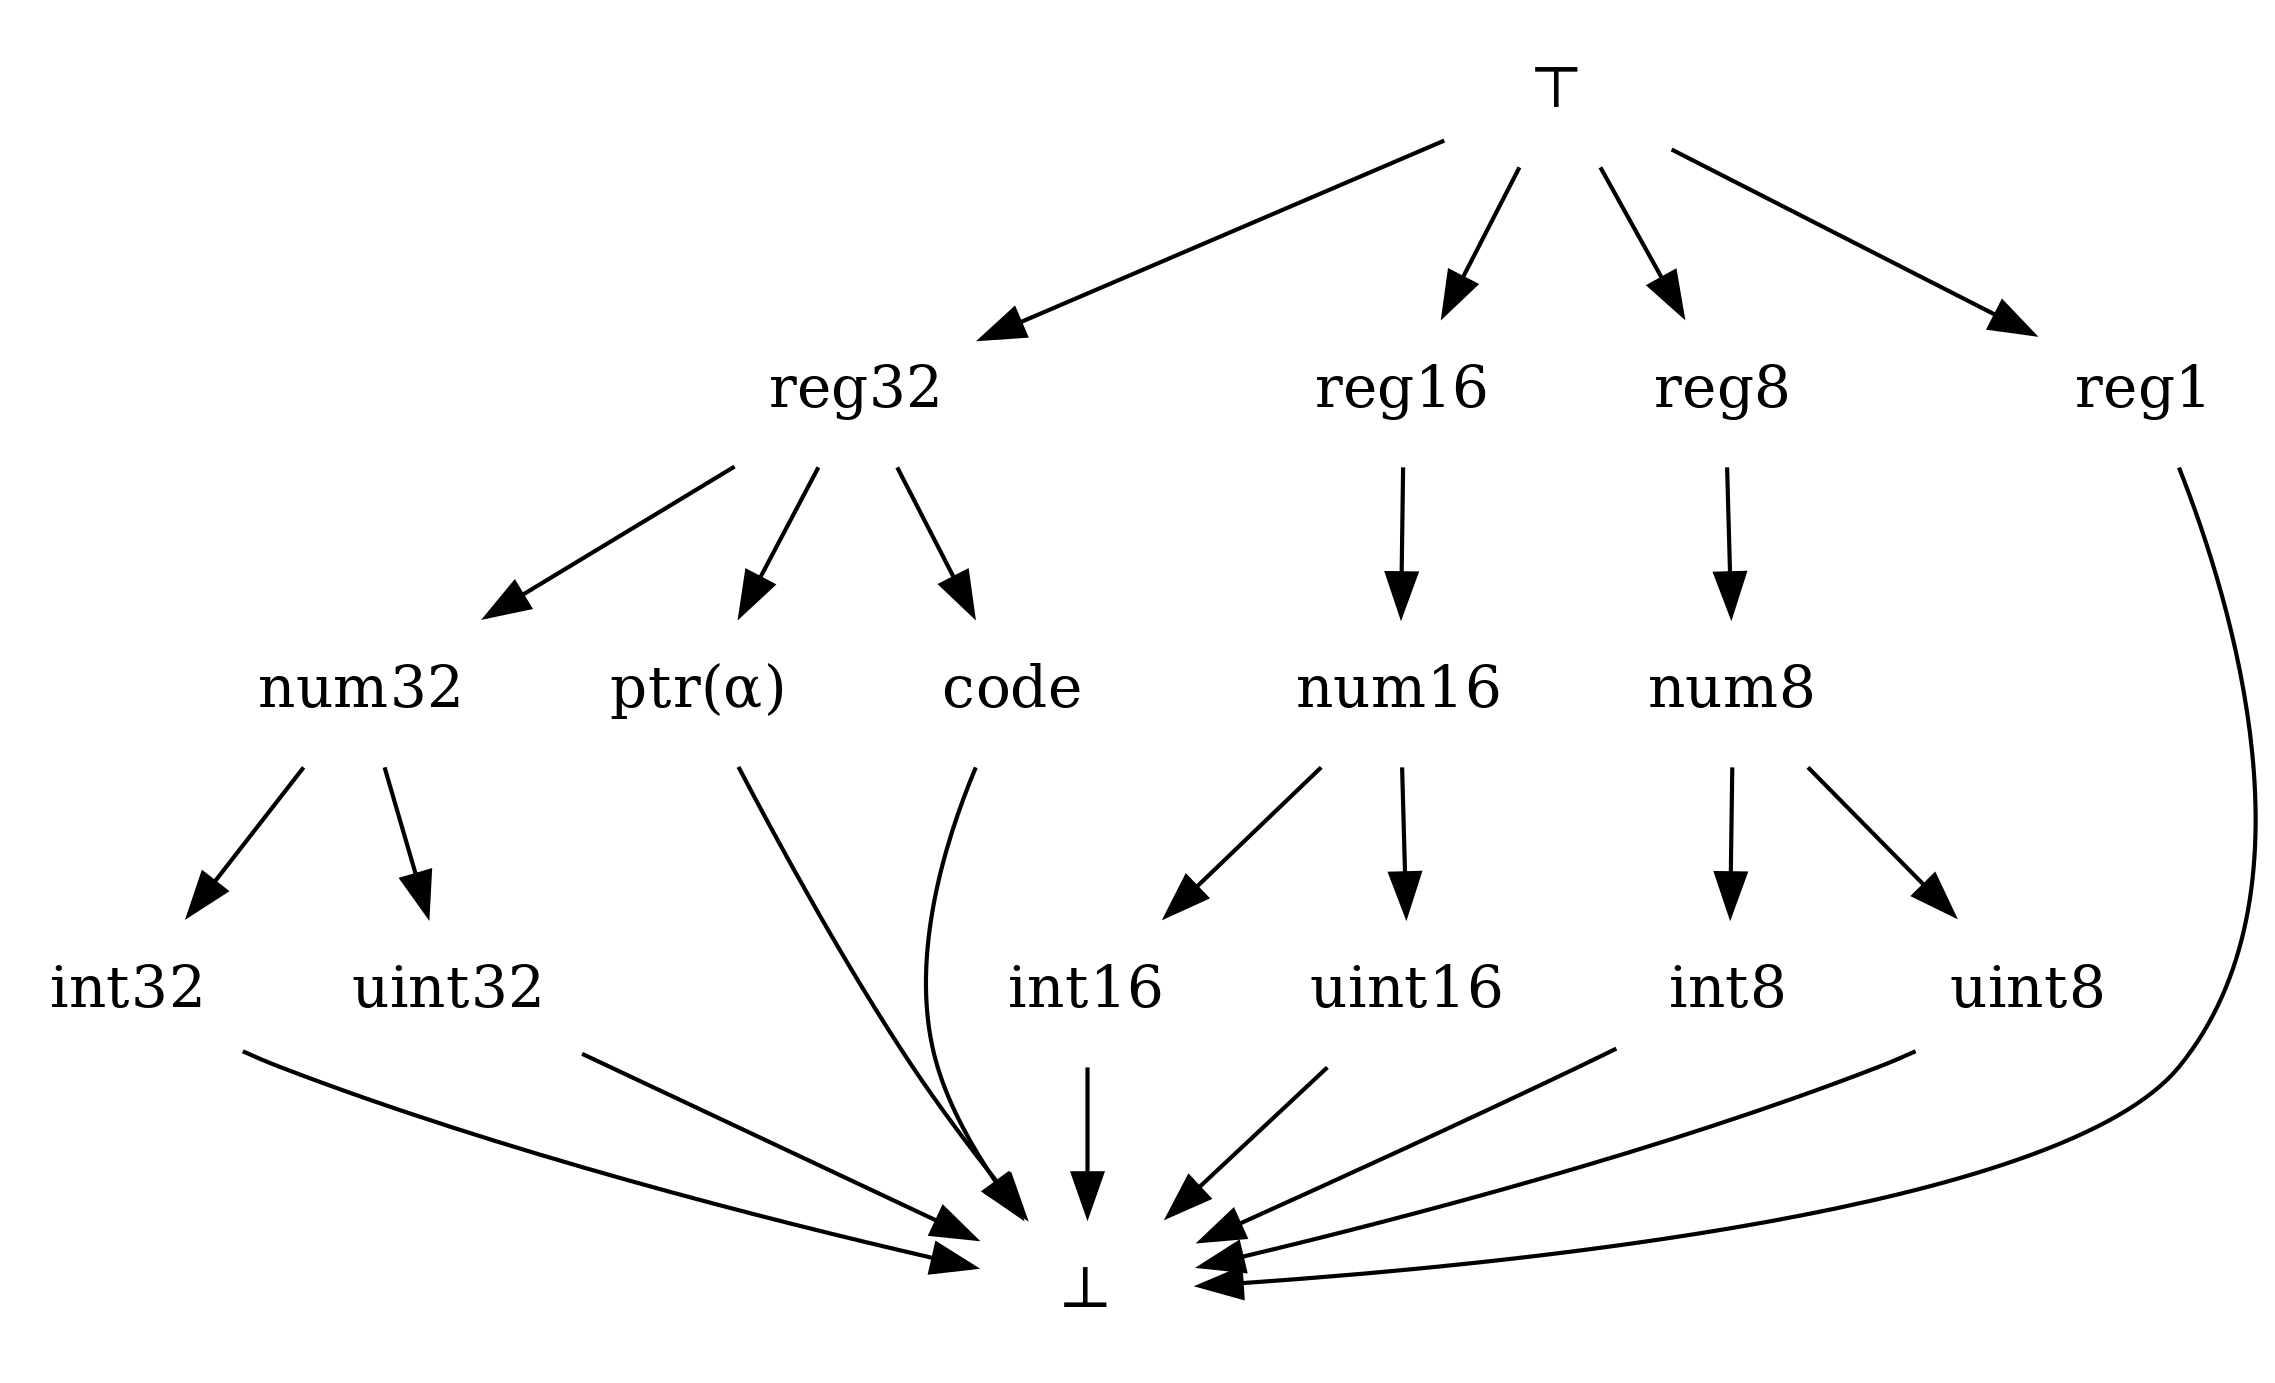
\includegraphics[width=0.45\textwidth]{inc/tie_primitive_type_lattice.png}
%	\caption{Primitive type lattice of TIE}
%	\label{fig:base_type_lattice}
%\end{teaserfigure}

% --- [ Title ] ----------------------------------------------------------------

\maketitle

% === [ Main matter ] ==========================================================

\question{QUESTION: Include abstract? The final paper will be around 6 pages.}

% TODO: change \include to \input

% === [ Introduction ] =========================================================

\section{Introduction}
\label{sec:introduction}

A compiler is a piece of software which translates human readable high-level programming languages (e.g. C) to machine readable low-level languages (e.g. Assembly). In the usual flow of compilation, code is lowered through a set of transformations from a high-level to a low-level representation. The decompilation process (originally referred to as reverse compilation \cite{reverse_comp}) moves in the opposite direction by lifting code from a low-level to a high-level representation.

Decompilation enables source code reconstruction of binary applications and libraries. Both security researchers and software engineers may benefit from decompilation as it facilitates analysis, modification and reconstruction of object code. The applications of decompilation are versatile, and may include one of the following uses:

\begin{itemize}
	\item Analyze malware
	\item Recover source code
	\item Migrate software from legacy platforms or programming languages
	\item Optimize existing binary applications
	\item Discover and mitigate bugs and security vulnerabilities
	\item Verify compiler output with regards to correctness
	\item Analyze proprietary algorithms
	\item Improve interoperability with other software
	\item Add new features to existing software
\end{itemize}

As recognized by Edsger W. Dijkstra in his 1972 ACM Turing Lecture (an extract from which is presented in figure \ref{fig:dijkstra_lecture}) one of the most powerful tools for solving complex problems in Computer Science is the use of abstractions and separation of concerns. This paper explores a compositional approach to decompilation which facilitates abstractions to create a pipeline of self-contained components. Since each component interacts through language-agnostic interfaces (well-defined input and output) they may be written in a variety of programming languages. Furthermore, for each component of the decompilation pipeline there may exist multiple implementations with their individual strengths and weaknesses. The end user (e.g. malware analyst, security researcher, reverse engineer) may select the components which solves their task most efficiently.

\begin{figure}[htbp]
	\begin{quote}
		\textit{``We all know that the only mental tool by means of which a very finite piece of reasoning can cover a myriad cases is called ``abstraction''; as a result the effective exploitation of their powers of abstraction must be regarded as one of the most vital activities of a competent programmer. In this connection it might be worthwhile to point out that the purpose of abstracting is not to be vague, but to create a new semantic level in which one can be absolutely precise. Of course I have tried to find a fundamental cause that would prevent our abstraction mechanisms from being sufficiently effective. But no matter how hard I tried, I did not find such a cause. As a result I tend to the assumption -- up till now not disproved by experience -- that by suitable application of our powers of abstraction, the intellectual effort needed to conceive or to understand a program need not grow more than proportional to program length.''} \cite{abstractions_quote}
	\end{quote}
	\caption{An extract from the ACM Turing Lecture given by Edsger W. Dijkstra in 1972.}
	\label{fig:dijkstra_lecture}
\end{figure}

\pagebreak % <layout>

% --- [ Project Aim and Objectives ] -------------------------------------------

\subsection{Project Aim and Objectives}
\label{sec:intro_project_aim_and_objectives}

The aim of this project is to facilitate decompilation workflows using composition of language-agnostic decompilation passes; specifically the reconstruction of high-level control structures and, as a future ambition, expressions.

To achieve this aim, the following objectives have been identified:

\begin{enumerate}
	\item Review traditional decompilation techniques, including control flow analysis and data flow analysis.
	\label{itm:obj_review_decomp_techniques}
	\item Critically evaluate a set of Intermediate Representations (IRs), which describes low-, medium- and high-level language semantics, to identify one or more suitable for the decompilation pipeline.
	\label{itm:obj_review_suitable_ir}
	\item Analyse the formal grammar (language specification) of the IR to verify that it is unambiguous. If the grammar is ambiguous or if no formal grammar exists, produce a formal grammar. This objective is critical for language-independence, as the IR works as a bridge between different programming languages.
	\label{itm:obj_formal_ir}
	\item Determine if any existing library for the IR satisfies the requirements; and if not develop one. The requirements would include a suitable in-memory representation, and support for on-disk file storage and arbitrary manipulations (e.g. inject, delete) of the IR.
	\label{itm:obj_ir_library}
	\item Design and develop components which identify the control flow patterns of high-level control structures using control flow analysis of the IR.
	\label{itm:obj_control_flow_analysis_component}
	\item Develop tools which perform one or more decompilation passes on a given IR. The tools will be reusable by other programming language environments as their input and output is specified by a formally defined IR.
	\label{itm:obj_decomp_pass_tool}
	\item As a future ambition, design and develop components which perform expression propagation using data flow analysis of the IR.
	\label{itm:obj_data_analysis_library}
\end{enumerate}

% --- [ Deliverables ] ---------------------------------------------------------

\subsection{Deliverables}
\label{sec:intro_deliverables}

The source code and the report of this project have been released into the public domain\footnote{CC0 1.0 Universal: \url{https://creativecommons.org/publicdomain/zero/1.0/}} and are made available on GitHub.

The following document has been produced:

\begin{itemize}
	\item Project report; see objective~\ref{itm:obj_review_decomp_techniques} and \ref{itm:obj_review_suitable_ir} \\ \url{https://github.com/decomp/decompilation}
\end{itemize}

And the following system artefacts have been developed:

\begin{itemize}
	\item Library for interacting with LLVM IR (\textit{work in progress}); see objective~\ref{itm:obj_ir_library} \\ \url{https://github.com/llir/llvm}
	\item Control flow graph generation tool; see objective~\ref{itm:obj_control_flow_analysis_component} \\ \url{https://github.com/decomp/ll2dot}
	\item Subgraph isomorphism search algorithms and related tools; see objective~\ref{itm:obj_control_flow_analysis_component} \\ \url{https://github.com/decomp/graphs}
	\item Control flow recovery tool; see objective~\ref{itm:obj_decomp_pass_tool} \\ \url{https://github.com/decomp/restructure}
	\item Go code generation tool (\textit{proof of concept}); see objective~\ref{itm:obj_decomp_pass_tool} \\ \url{https://github.com/decomp/ll2go}
	\item Go post-processing tool; see objective~\ref{itm:obj_decomp_pass_tool} \\ \url{https://github.com/decomp/go-post}
\end{itemize}

% --- [ Disposition ] ----------------------------------------------------------

\subsection{Disposition}

This report details every stage of the project from conceptualisation to successful completion. It follows a logical structure and outlines the major stages in chronological order. A brief summary of each section is presented in the list below.

\begin{itemize}
	\item Section~\ref{sec:introduction} - \textbf{Introduction} \\ \textit{Introduces the concept of decompilation and its applications, outlines the project aim and objectives, and summarises its deliverables.}
	\item Section~\ref{sec:literature_review} - \textbf{Literature Review} \\ \textit{Details the problem domain, reviews traditional decompilation techniques, and evaluates potential intermediate representations for the decompilation pipeline of the project.}
	\item Section~\ref{sec:related_work} - \textbf{Related Work} \\ \textit{Evaluates projects for translating native code to LLVM IR, and reviews the design of modern decompilers.}
	\item Section~\ref{sec:methodology} - \textbf{Methodology} \\ \textit{Surveys methodologies and best practices for software construction, and relates them to the specific problem domain.}
	\item Section~\ref{sec:requirements} - \textbf{Requirements} \\ \textit{Specifies and prioritises the requirements of the project artefacts.}
	\item Section~\ref{sec:design} - \textbf{Design} \\ \textit{Discusses the system architecture and the design of each component, motivates the choice of core algorithms and data structures, and highlights strengths and limitations of the design.}
	\item Section~\ref{sec:implementation} - \textbf{Implementation} \\ \textit{Discusses language considerations, describes the implementation process, and showcases how set-backs were dealt with.}
	\item Section~\ref{sec:verification} - \textbf{Verification} \\ \textit{Describes the approaches taken to validate the correctness, performance and security of the artefacts.}
	\item Section~\ref{sec:evaluation} - \textbf{Evaluation} \\ \textit{Assesses the outcome of the project and evaluates the artefacts against the requirements.}
	\item Section~\ref{sec:conclusion} - \textbf{Conclusion} \\ \textit{Summarises the project outcomes, presents ideas for future work, reflects on personal development, and concludes with an attribution to the key idea of this project.}
\end{itemize}


% === [ Background ] ===========================================================

\section{Background}

This section provides a brief background on important terminology and concepts related to type analysis.

\question{QUESTION: Should the Background section be merged with the Type Analysis section?}

% === [ Subsections ] ==========================================================

% --- [ Static Single Assignment ] ---------------------------------------------

\subsection{Static Single Assignment}

Static Single Assignment (SSA) form is a property of an intermediate representation (IR) in which each variable is defined before use and assigned exactly once. SSA-form is commonly used in the IR of compilers as it facilitates data flow analysis and simplifies some optimization passes (e.g. dead code elimination).

% TODO: Reformulate and perhaps move?

Within type analysis, SSA-form help distinguish distinct variables stored in the same register by tracking their live ranges. For instance, in the running example (see listing \ref{fig:local_variable_example_asm} of appendix \ref{app:local_variable_example}) the \texttt{eax} register is defined at lines 15, 19, 23 and 25, and refers to different variables of different types. When converted to SSA-form each of these assignments would be to a unique \textit{version} of the \texttt{eax} variable; e.g. \texttt{\%eax.0}, \texttt{\%eax.1}, \texttt{\%eax.2}, etc.

Multiple assignments to the same source variable are represented in SSA-form using $\Phi$ (\textit{Phi}) instructions (also known as $\Phi$ functions). A $\Phi$ instruction essentially merges (joins) data flow, such that the resulting value of the $\Phi$ instruction depend on the branch taken in the control flow graph (as further illustrated in figure \ref{fig:phi_node_semantics} and \ref{fig:ssa_form}).

\begin{figure}[htbp]
	\centering
	\begin{subfigure}[ht]{0.18\textwidth}
		\centering
		\lstinputlisting[language=c, style=go, breaklines=false]{inc/ssa.c}
		\caption{C source code.}
		\label{fig:c_source_phi}
	\end{subfigure}
	\qquad
	\begin{subfigure}[ht]{0.25\textwidth}
		\centering
		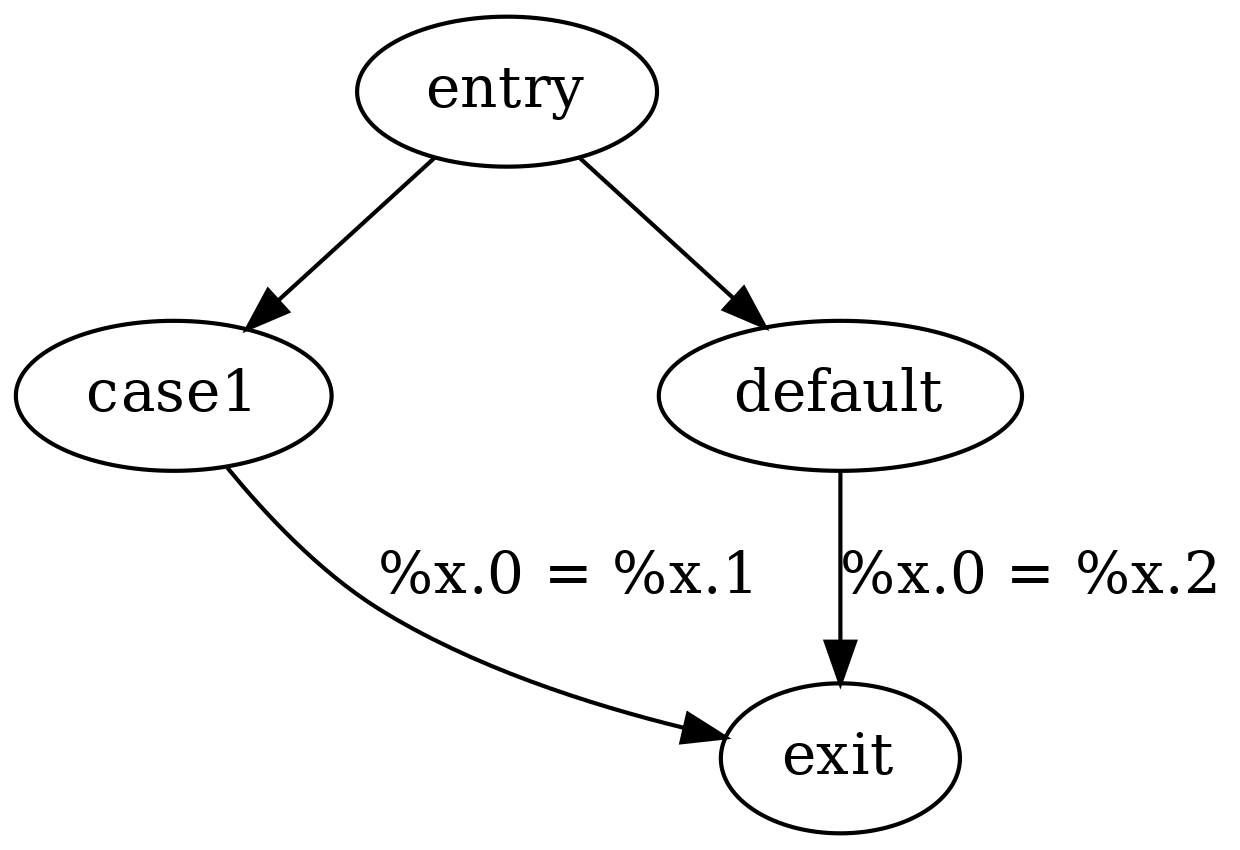
\includegraphics[width=\textwidth]{inc/phi.png}
		\caption{$\Phi$-node semantics: value of \texttt{\%x.0} in \texttt{\%exit} basic block depend on branch taken.}
		\label{fig:phi_node_semantics}
	\end{subfigure}
	\begin{subfigure}[ht]{0.50\textwidth}
		\lstinputlisting[language=llvm, style=nasm, breaklines=false]{inc/ssa.ll}
		\caption{LLVM IR in SSA-form: each variable is assigned exactly once.}
		\label{fig:ssa_form}
	\end{subfigure}
	\caption{C source code converted to LLVM IR in SSA-form and associated CFG illustrating $\Phi$-node semantics..}
\end{figure}

% --- [ Type Lattice ] ---------------------------------------------------------

\subsection{Type Lattice}

A type lattice may be thought of as a set of subtyping relationships, represented as a directed graph from the \textit{top} type $\top$ to the \textit{bottom} type $\bot$; where every type is a subtype of $\top$, and no type is a subtype of $\bot$.

\begin{itemize}
	\item $\top$: any type
	\item $\bot$: inconsistent type
\end{itemize}

In the type primitive type lattice of TIE (see figure \ref{fig:primitive_type_lattice}) for instance, both signed and unsigned 32-bit integers (\texttt{int32} and \texttt{uint32}, respectively) are subtypes of 32-bit integers (\texttt{num32}) \cite{tie_reverse_engineering_of_types}.

\begin{figure}[htbp]
	\centering
	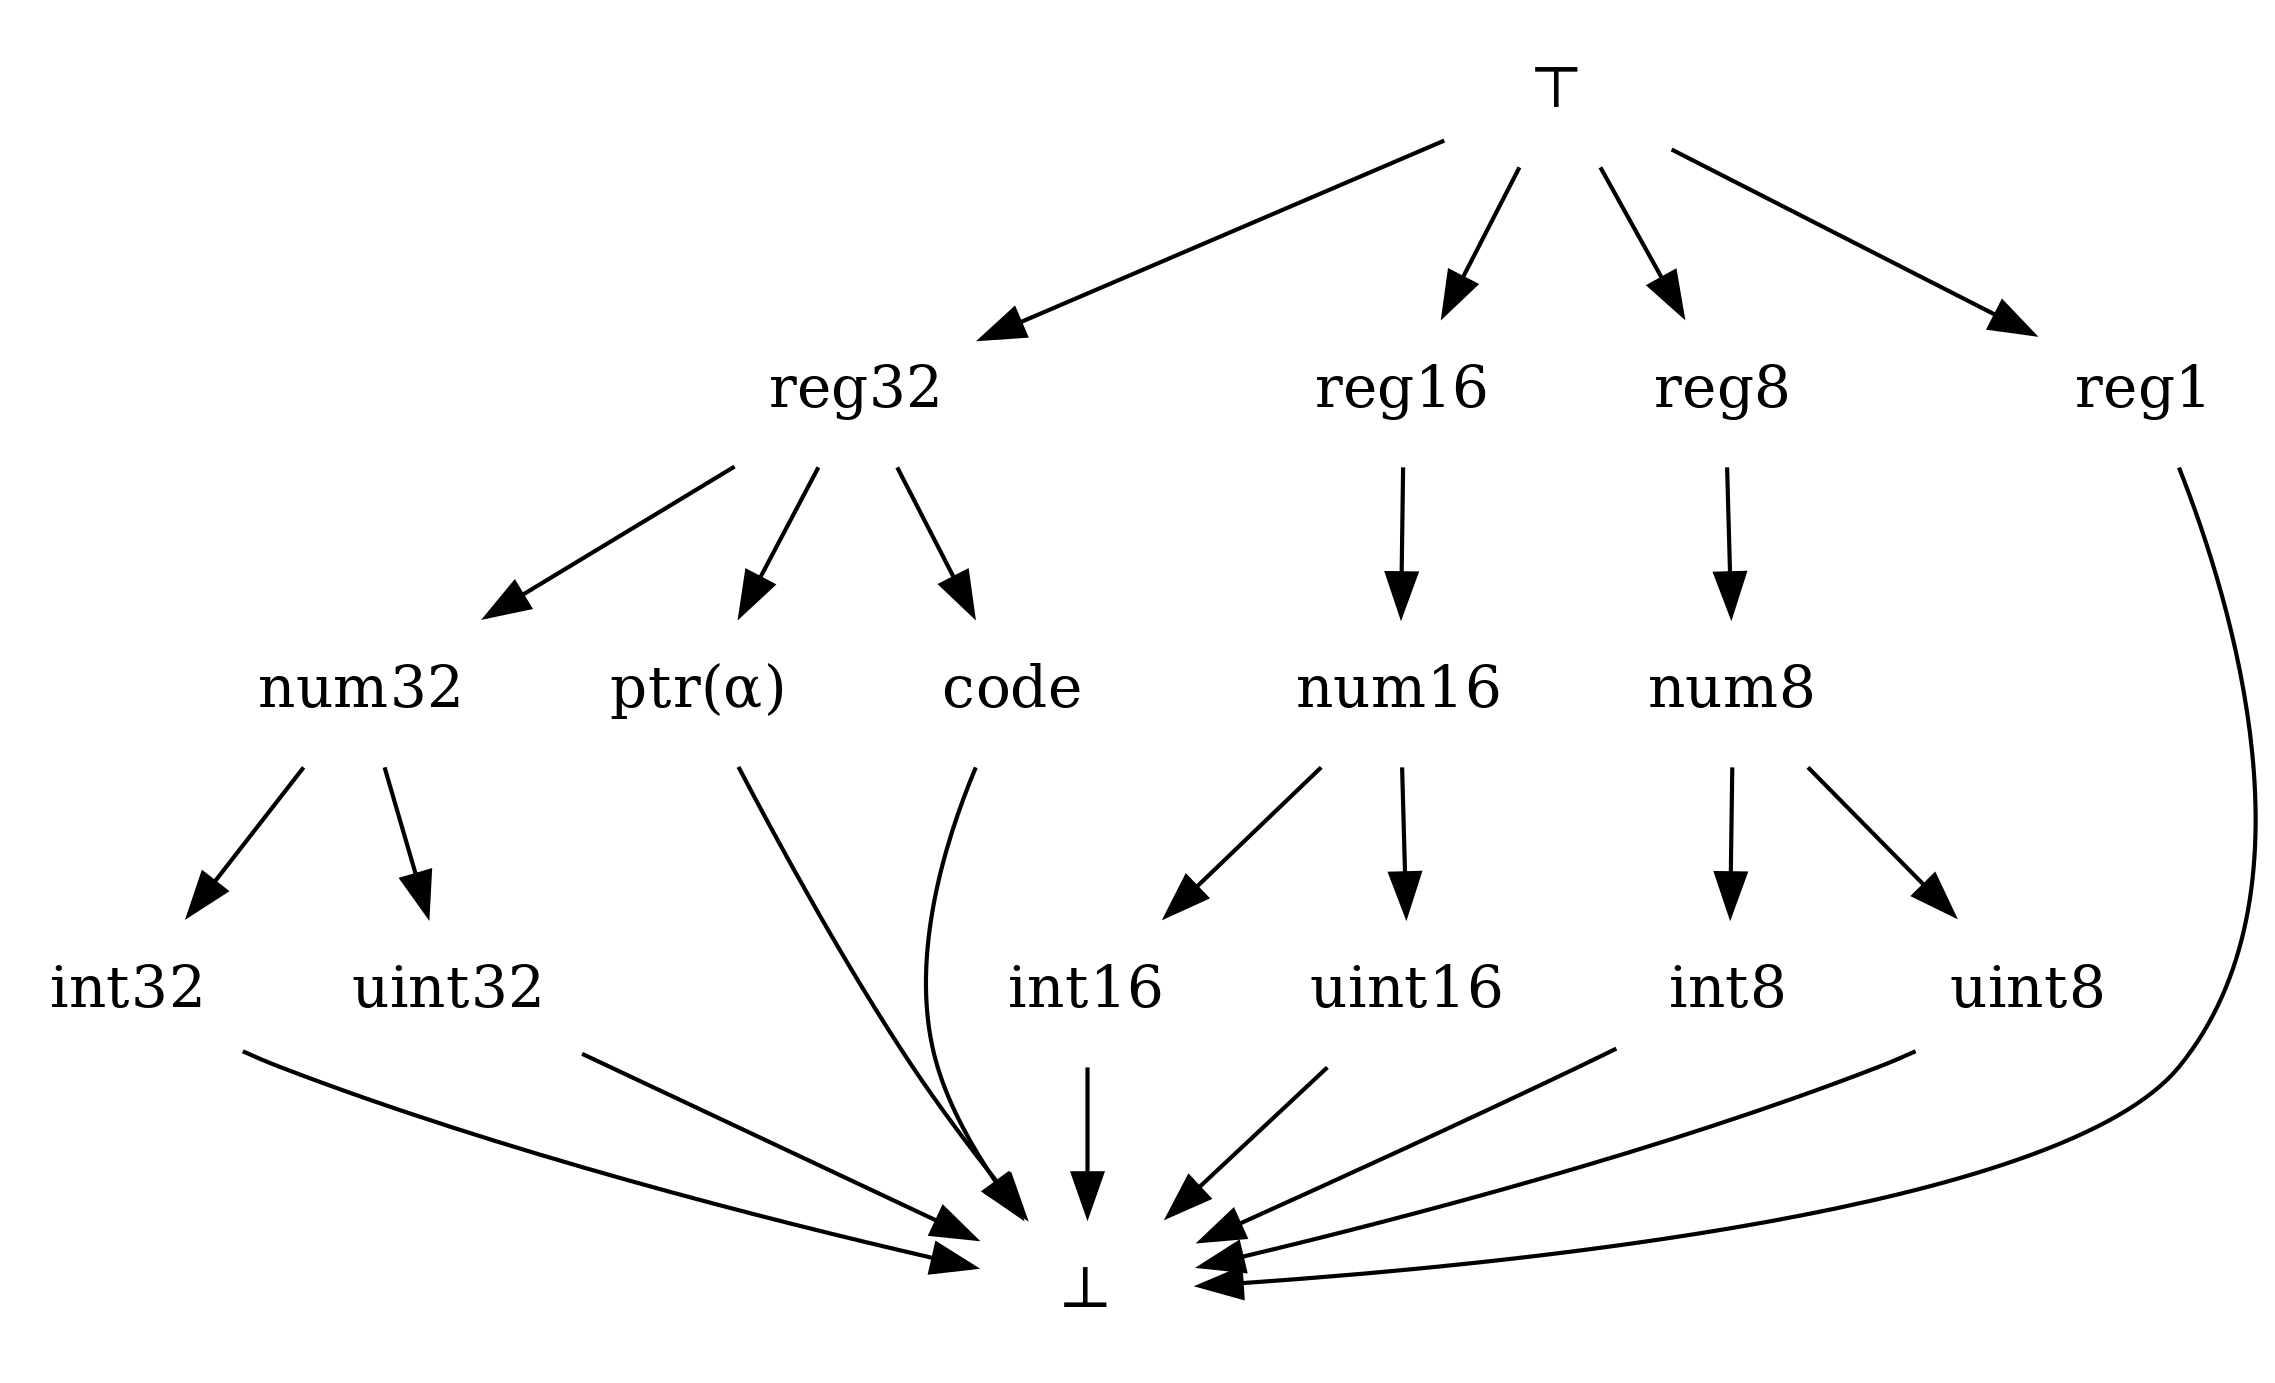
\includegraphics[width=0.40\textwidth]{inc/tie_primitive_type_lattice.png}
	\caption{Primitive type lattice of TIE.}
	\label{fig:primitive_type_lattice}
\end{figure}

In the context of type recovery, a type lattice may be used to specify the set of possible types for a variable through upper and lower bounds; thus imposing type constraints on the variable.

% --- [ Static Analysis ] ------------------------------------------------------

\subsection{Static Analysis}

\todo{TODO: describe relevant aspects of static analysis. Covers all code paths but does not known concrete values of pointers, and some techniques of memory graph analysis are thus limited. (Verify if this is actually true, claimed in Type Inference on Executables. However Symbolic execution may mitigate this limitation even in static analysis.)} \cite{type_inference_on_executables}

% --- [ Dynamic Analysis ] -----------------------------------------------------

\subsection{Dynamic Analysis}

\todo{TODO: describe relevant aspects of dynamic analysis. Does not cover all code paths (as static analysis does), but still relevant and widely used in Malware forensics. Particularly useful for memory access analysis, to recover structure types as their members are accessed during execution.} \cite{dynstruct}


% === [ Variable Recovery ] ====================================================

\section{Variable Recovery}

\todo{TODO: add meta-text; prior to type analysis, the set of variables must first be recovered, as they are to be assigned types.}

% --- [ Value Set Analysis ] ---------------------------------------------------

\subsection{Value Set Analysis}

\todo{TODO: describe value set analysis}

upper bound, lower bound and stride for memory locations.


% --- [ Function signature recovery ] ------------------------------------------

\subsection{Function signature recovery}

\todo{TODO: add note about call conventions}

% TODO: rephrase.

The following set of steps are used for function signature recovery (function parameters and returns arguments) in SecondWrite \cite{second_write_scalable_type_detection}.

\begin{enumerate}
	\item assume all registers are arguments and no register are return arguments.
	\item registers written to are potential return arguments.
	\item callee saved registers (through push in function prologue and pop in function epilogue) (\textit{DeadStores}) are pruned from potential return set.
	\item prune arguments not actually used (e.g. not part of \textit{DeadStore} or PHI instructions).
	\item prune return registers not actually used by callers.
\end{enumerate}

% === [ Type Recovery ] ========================================================

\section{Type Recovery}

% Key: many problems in binary analysis can be seen as subproblems of type analysis.

% binary analysis,

% floating-point stack
%    - track stack top (indirect calls/external calls)
% pointer analysis
%    - global memory region
%    - stack memory region
%    - heap memory region
% structures/arrays

\todo{TODO: give introduction to type recovery as part of type analysis of low-level code.} \cite{mycroft_type_based_decompilation}

\paragraph{Value-based type inference} \todo{TODO: describe value-based type inference. E.g. if value is \texttt{42}, infer that it is an integer, if value is \texttt{0x401005} infer that it is a pointer. Bring up problems with this approach, misclassification.} \cite{type_inference_on_executables}

\paragraph{Flow-based type inference}

\todo{TODO: describe type inference, Algorithm W} \cite{milner_algorithmw}

\paragraph{Type propagation}

\todo{TODO: describe type propagation, type constraints, forward and backward propagation, constraint solving}

\paragraph{Unification}

\todo{TODO: describe the unification step, as many algorithms rely on this to discover structure types, etc.}

\paragraph{Instruction type sources}

Also known as type revealing instruction.

\todo{TODO: describe type revealing instructions. Infer from the instruction that the operand is of integer type, memory, floating-point, etc.}

\paragraph{Function type sources} Type information derived for arguments in calls to functions with known functions signatures (e.g. those of the standard library). \cite{type_inference_on_executables}

\paragraph{Type sink} A type sink is a type which can be resolved directly and is known to be correct. For instance, types for arguments inferred from function type sources.

\paragraph{Pointer analysis}

\todo{TODO: give brief introduction to pointer analysis, points-to sets, pointer aliasing, and the technique to merge call sites such that memory allocated at different allocation call sites (e.g. calls to \texttt{malloc}) may have the same type if proven that through type propagation, that the returned pointers are used at other parts of the program for the same variables.}

% === [ Evaluation Metrics ] ===================================================

\section{Evaluation Metrics}

\todo{TODO: add note on the use of debug information.}

\todo{TODO: mention that SPEC2006 and Coreutils are often used in benchmarks.}

To enable objective comparison of different type recovery methods, a shared set of evaluation metrics are required. For this purpose, TIE proposed two evaluation metrics: \textit{distance} and \textit{conservativeness} \cite{tie_reverse_engineering_of_types}.

% --- [ Distance ] -------------------------------------------------------------

\subsection{Distance}

The distance in height between the recovered and the source type in the primitive type lattice (see figure \ref{fig:base_type_lattice}) for subtypes (e.g. \texttt{int32} is a subtype of \texttt{num32} at distance 1), and the maximum lattice height otherwise.

% --- [ Conservativeness ] -----------------------------------------------------

\subsection{Conservativeness}

Reports whether the source type exists within the type range (lower and upper bound) of the recovered type.

The distance measurement as defined by TIE did not distinguish between multi-level pointers (e.g. \texttt{int*} and \texttt{int**} are equivalent, i.e. on the same level in the type lattice). Thus SecondWrite proposed a refinement to measure the ratio of between the recovered pointer level and the source pointer level \cite{second_write_scalable_type_detection}.

Other metrics have been proposed to compare class hierarchies.

% === [ Discussion ] ===========================================================

\section{Discussion}

% (Reminder: method, research results.)

\todo{TODO: critically assess results.}

% * make claims
% * interpret results (interpretation of your data)
%    - what limitations are there?
%    - can we depend on this?
%    - relevance to your research question?
%    - relevance to your field of study?

% === [ Conclusion ] ===========================================================

\section{Conclusion}

% --- [ Future Research ] ------------------------------------------------------

\subsection{Future Research}

As a future research topic, it would be very interesting to combine a variety of control flow recovery methods, and evaluate if they may facilitate each other to further improve control flow recovery.

Additional insights could be provided by a deeper evaluation which examines how the control flow recovery methods deal with irreducible graphs, as produces by various compiler optimisations (e.g. jump threading).


% TODO: skip? \cite{bintype}
% TODO: skip? \cite{polymorphic_type_inference_for_machine_code}

% === [ Back matter ] ==========================================================

% --- [ References ] -----------------------------------------------------------

\clearpage

\bibliography{references}

% --- [ Appendices ] -----------------------------------------------------------

% === [ Appendix ] =============================================================

\onecolumn

\appendix
\setcounter{secnumdepth}{0}
\section{Appendices}
\setcounter{secnumdepth}{3}
\renewcommand{\thesubsection}{\Alph{subsection}}

% --- [ Running Example ] ------------------------------------------------------

\subsection{Running Example}
\label{app:running_example}

\begin{figure}[htbp]
	\centering
	\begin{subfigure}[ht]{0.3\textwidth}
		\centering
		\lstinputlisting[language=c, style=go, breaklines=false]{inc/example.c}
		\caption{Example C source code.}
		\label{fig:running_example_c}
	\end{subfigure}
	\qquad
	\begin{subfigure}[ht]{0.6\textwidth}
		\centering
		\lstinputlisting[language=nasm, style=nasm, breaklines=false]{inc/example.asm}
		\caption{Corresponding assembly code in NASM syntax.}
		\label{fig:running_example_asm}
	\end{subfigure}
	\caption{Running example used to illustrate different aspects of variable recovery and type analysis.}
	\label{fig:running_example}
\end{figure}


\end{document}
